\section{Przedstawienie problemu}

\subsection{Internet rzeczy}
W ostatnich latach obserwujemy gwałtowny wzrost automatyzacji i cyfryzacji. (statystyka - \cite{statistaconnecteddevices}) Inteligentne urządzenia możemy znaleźć już w wielu miejscach: w strefach przemysłowych, gdzie ich zadaniem jest ulepszenie i ułatwienie procesu produkcji, na naszych drogach, gdzie pomagają w odkorkowywaniu miast. Obecnie coraz większą popularnością cieszą się one również w naszych domach (statystyka - \cite{iotstatistasmarthome}), najczęściej pod postacią drobnych urządzeń znanych producentów. Takie urządzenia pomagają nam w automatyzacji codziennych czynności: zdalne zarządzanie światłem, kontrola poboru prądu, klimatyzacja i ogrzewanie, ale również mogą monitorować nasze bezpieczeństwo, przykładowo z wykorzystaniem czujnika zalania w łazience. Z użyciem grupy czujników i sensorów oraz elementów wykonawczych takich jak wentylatory, grzejniki, żarówki, przełączniki, głośniki i wiele innych możemy zautomatyzować wiele codziennych czynności, poprawić komfort naszego życia jak i ograniczyć zużycie zasobów.\\

Dla przykładu, inteligentne termostaty uczą się naszych zwyczajów i dostosowują ogrzewanie do naszego trybu życia, obniżając temperaturę, kiedy jesteśmy poza domem, co przekłada się na znaczne oszczędności energetyczne. Znając lokalizację domowników system może wyłączyć ogrzewanie jeżeli dom stoi pusty i zawczasu je włączyć gdy się zbliżamy. Możemy poprawić zużycie prądu, ogrzewając wodę w bojlerze jedynie w nocy gdy taryfa jest bardziej opłacalna czy ustawić harmonogram podlewania roślin w ogrodzie. Opcji jest multum.\\

Dodatkowo, inteligentne systemy mogą poprawić jakość życia osób starszych lub niepełnosprawnych, umożliwiając im większą samodzielność. Za pomocą prostych komend głosowych mogą one kontrolować różne urządzenia w domu, od telewizora po żaluzje, co sprawia, że ich codzienne życie staje się łatwiejsze i bardziej komfortowe.\\

Na rynku pojawiają się również inteligentne urządzenia kuchenne, takie jak lodówki, które monitorują stan zapasów i mogą automatycznie zamawiać produkty spożywcze, kiedy zaczynają się kończyć, czy piekarniki, które dostosowują czas i sposób pieczenia do rodzaju potrawy. To wszystko sprawia, że nasze życie staje się nie tylko wygodniejsze, ale także bardziej ekologiczne, ponieważ dzięki precyzyjnej kontroli zużycia możemy znacznie zmniejszyć nasz ślad węglowy.\\

Automatyzacja i inteligentne urządzenia zmieniają sposób, w jaki żyjemy, pracujemy i odpoczywamy, oferując nam nowe możliwości i sprawiając, że nasz codzienny komfort jest na wyższym poziomie. W miarę rozwoju technologii możemy spodziewać się jeszcze większej integracji inteligentnych systemów w naszym życiu codziennym, co otwiera przed nami fascynujące perspektywy.

\newpage

\subsection{Zamknięte oprogramowanie}
Całość brzmi świetnie: lepiej, szybciej, więcej, wygodniej. Niestety wiele urządzeń popularnych producentów wykorzystuje zamknięte oprogramowanie. Często musimy używać wiele aplikacji różnych producentów aby sterować wszystkimi urządzeniami w naszym domu. To jednak problem jedynie wygody jednak zamknięte oprogramowanie rodzi jeszcze jeden o wiele poważniejszy. Nie posiadamy kontroli ani wiedzy w jaki sposób te urządzenia komunikują się z infrastrukturą producenta. Jakie dane wysyłają i czy nie posiadają luk bezpieczeństwa. Co w przypadku gdy te urządzenia są źle zaprojektowane i posiadają podatności za pośrednictwem których osoby trzecie mogą przejąć kontrolę nad całą naszą siecią domową. Prosta żarówka którą możemy zdalnie włączyć, nie zależnie od tego czy jesteśmy w salonie naszego domu czy na drugim końcu świata, musi komunikować się z serwerami producenta o których wiemy niewiele.\\

Znane są przypadki gdy inteligentne odkurzacze czy domowe dzwonki odmawiały posłuszeństwa z powodu awarii serwerów. (artykuł BBC - \cite{amazonoutage}) Dodatkowo, te awarie mogą prowadzić nie tylko do tymczasowego braku dostępu do funkcji urządzenia, ale również do trwałej utraty danych lub nieautoryzowanego do nich dostępu przez osoby trzecie. Bez odpowiedniej transparentności i kontroli nad tym, jak nasze urządzenia komunikują się z zewnętrznymi serwerami, stajemy się podatni na różnego rodzaju ataki cybernetyczne. To, co wydaje się być wygodą, może przekształcić się w poważne zagrożenie dla naszej prywatności i bezpieczeństwa.\\

Otwarte oprogramowanie nie tylko zwiększa transparentność działania urządzeń, umożliwiając użytkownikom lepsze zrozumienie procesów zachodzących w ich sprzęcie, ale również pozwala na szybsze wykrywanie i łatanie ewentualnych luk bezpieczeństwa przez społeczność. (GNU Manifesto - \cite{gnumanifesto})\\

Stosowanie lokalnych protokołów komunikacyjnych, które nie wymagają stałego połączenia z serwerami producenta zmniejsza ryzyko awarii i nieautoryzowanego dostępu do naszych danych. Przykładem mogą być systemy, które działają w pełni wewnątrz sieci domowej, bez potrzeby wysyłania danych na zewnątrz.\\

Ważne jest, aby konsumenci byli świadomi tych zagrożeń i domagali się od producentów większej przejrzystości oraz bezpieczeństwa. Wymaganie od producentów wdrażania standardów otwartego oprogramowania oraz lokalnych protokołów komunikacyjnych może przyczynić się do zwiększenia bezpieczeństwa i prywatności w naszych domach. Tylko w ten sposób możemy mieć pewność, że korzyści płynące z inteligentnego domu nie będą miały negatywnych konsekwencji dla naszego bezpieczeństwa.

\newpage

\subsection{Protokoł MQTT}
Stworzony w 1999 roku prosty i lekki protokół komunikacyjny MQTT (Message Queuing Telemetry Transport) jest przeznaczony dla urządzeń niewymagających wysokiej przepustowości. Protokół ten przeszedł kilka istotnych aktualizacji, w tym wersje 3.1 (dokumentacja - \cite{mqtt3spec}) i 5.0 (dokumentacja - \cite{mqtt5spec}), które wprowadziły nowe funkcje i usprawnienia, takie jak lepsze zarządzanie jakością usług, rozszerzone możliwości zabezpieczeń oraz wsparcie dla bardziej złożonych scenariuszy komunikacyjnych. (artykuły HiveMQ - \cite{mqtt5part1}\cite{mqtt5part2}) MQTT jest szeroko wykorzystywany w IoT oraz wszędzie tam, gdzie wymagana jest oszczędność przepustowości i energii.

\subsubsection{Broker}
Architektura oparta o MQTT wymaga serwera na którym pracuje broker wiadomości implementujący protokół MQTT. Broker stanowi centralny punkt do którego łączą się wszyscy klienci. Przykładem brokera MQTT jest Eclipse Mosquitto. (dokumentacja - \cite{mosquittodocs})

\subsubsection{Topic}
Abstrakcyjne identyfikatory pomagające przesyłać wiadomości do konkretnych odbiorców. Nie istnieją fizycznie a publikacja i subskrypcja do nich nie wymaga uprzedniego ich utworzenia. Dany \tcbox{topic} można porównać do tablicy ogłoszeń którą każdy zainteresowany może zasubskrybować aby otrzymać powiadomienie za każdym razem gdy ktoś publikuje na niej nową wiadomość.\\

Aby otrzymać to powiadomienie klient musi, nie tylko wcześniej zasubskrybować dany \tcbox{topic}, ale również być na czas publikacji połączonym z brokerem. Jedynym wyjątkiem od tej zasady jest przypadek\\gdy \tcbox{topic} posiada \tcbox{retained message}.

\subsubsection{Retained message}
Jest to specjalny rodzaj wiadomości wysyłanej na dany \tcbox{topic} różniący się ustawioną flagą \tcbox{retained}. Broker zachowuje taką wiadomość i przesyła ją do klienta na moment subskrypcji tego \tcbox{topic}. Każdy \tcbox{topic} może mieć tylko jedną \tcbox{retained message}. Aby ją usunąć wymagana jest publikacja nowej wiadomości z flagą \tcbox{retained} oraz pustym \tcbox{payload}.

\subsubsection{Message payload}
Jest to ciąg znaków który wysyłany jest z każdą wysłaną wiadomością. Dla przykładowego \tcbox{topic} o nazwie temperatura może być to aktualna temperatura w pokoju wyrażona w stopniach Celsjusza.

\newpage

\subsubsection{Przykład wykorzystania}
Poniższe grafiki prezentują przykład użycia protokołu MQTT w praktyce. W przykładzie bierze udział troje urządzeń: termometr mierzący temperaturę w pokoju, sterownik ogrzewania mający za zadanie na podstawie zmierzonej temperatury włączać bądź wyłączać ogrzewanie oraz panel sterowania który dla uproszczenia został celowo wykluczony ze schematów.\\

1. Wpierw każde z urządzeń nawiązuje połączenie do brokera które pozostaje stale utrzymane na czas pracy urządzenia. W przypadku zerwania połączenia, urządzenie stara się je ponownie nawiązać ponieważ w innym razie jest wykluczone z komunikacji.\\\\
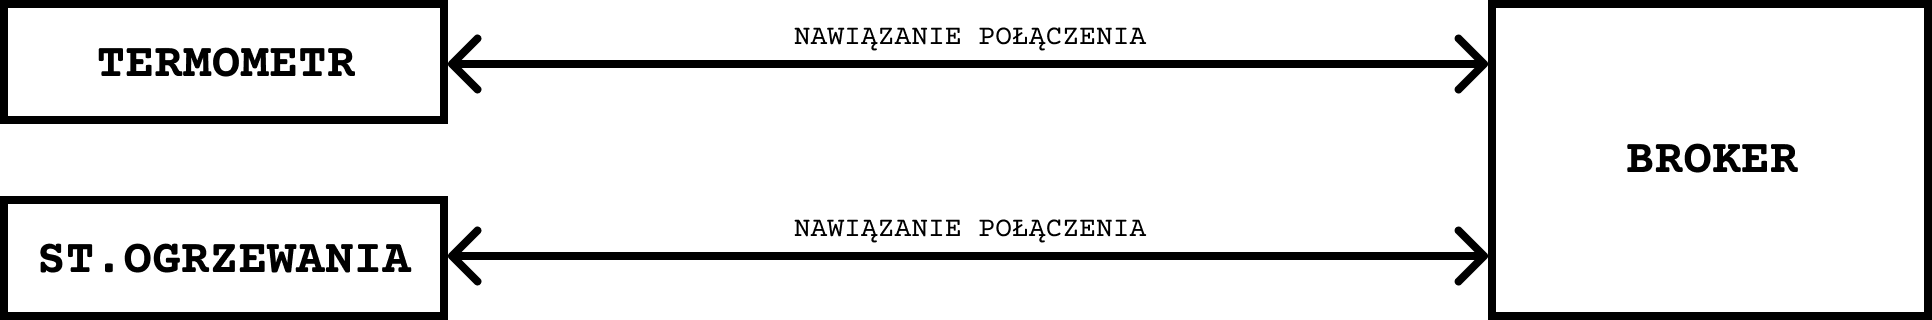
\includegraphics[scale=1.005]{mqtt1}\\\\

2. Po połączeniu każde urządzenie które tego potrzebuje subskrybuje interesujące je \tcbox{topic}. W tym przykładzie sterownik ogrzewania subskrybuje \tcbox{topic} temp. W tym momencie, jeżeli \tcbox{topic} temp posiadałby retained message, sterownik otrzymałby tą wiadomość dokładnie tak samo jakby była ona świeżo nadana. W innym przypadku sterownik nie znałby obecnej temperatury do momentu nadania jej przez termometr w kolejnym kroku.\\\\
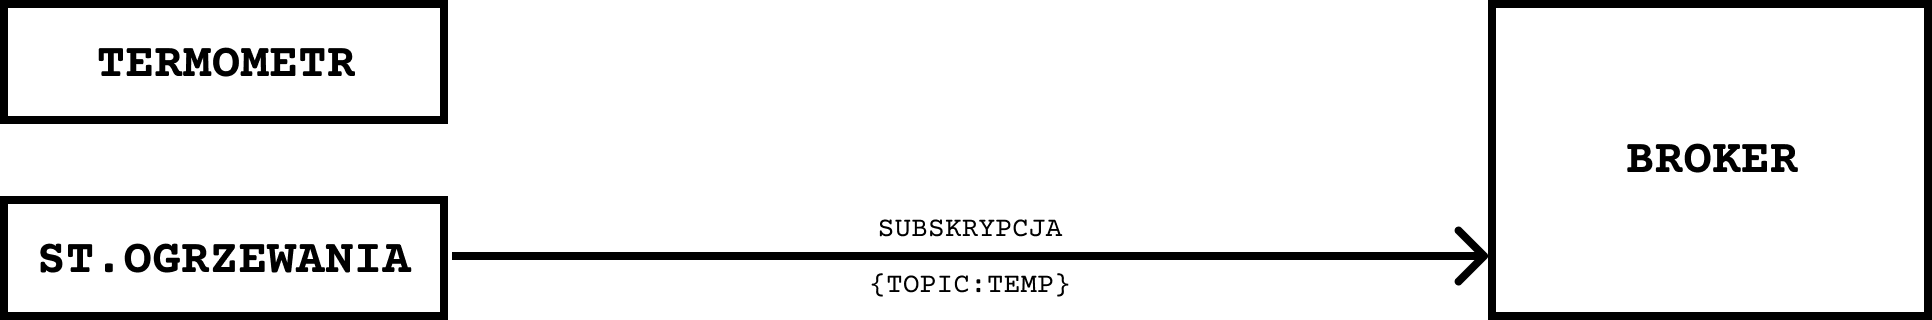
\includegraphics[scale=1.005]{mqtt2}\\\\

3. Termometr wysyła nową wiadomość na \tcbox{topic} temp z payload wynoszącym wartość zmierzonej temperatury. Ten krok powtarza się z określoną częstotliwością. W ten sposób \tcbox{topic} temp reprezentuje aktualną temperaturę w pokoju.\\\\
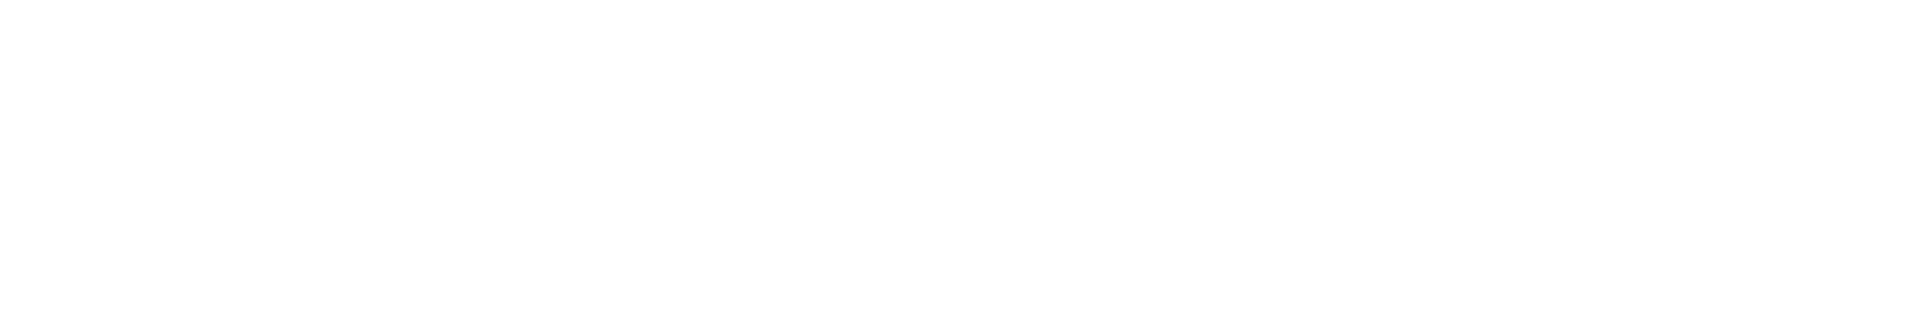
\includegraphics[scale=1.005]{mqtt3}\\\\

4. W odpowiedzi na publikację nowej wiadomości broker powiadamia każde urządzenie subskrybujące \tcbox{topic} temp. Po otrzymaniu aktualnej wartości sterownik może podjąć decyzję czy włączyć lub wyłączyć ogrzewanie w pokoju. Sam stan ogrzewania może być oddzielnym \tcbox{topic}, tak aby panel sterowania mógł wyświetlić informację czy jest ono włączone bądź nie: gdy sterownik włącza ogrzewanie publikuje 1 na \tcbox{topic} \tcbox{ogrz}, a gdy je wyłącza publikuje 0.\\\\
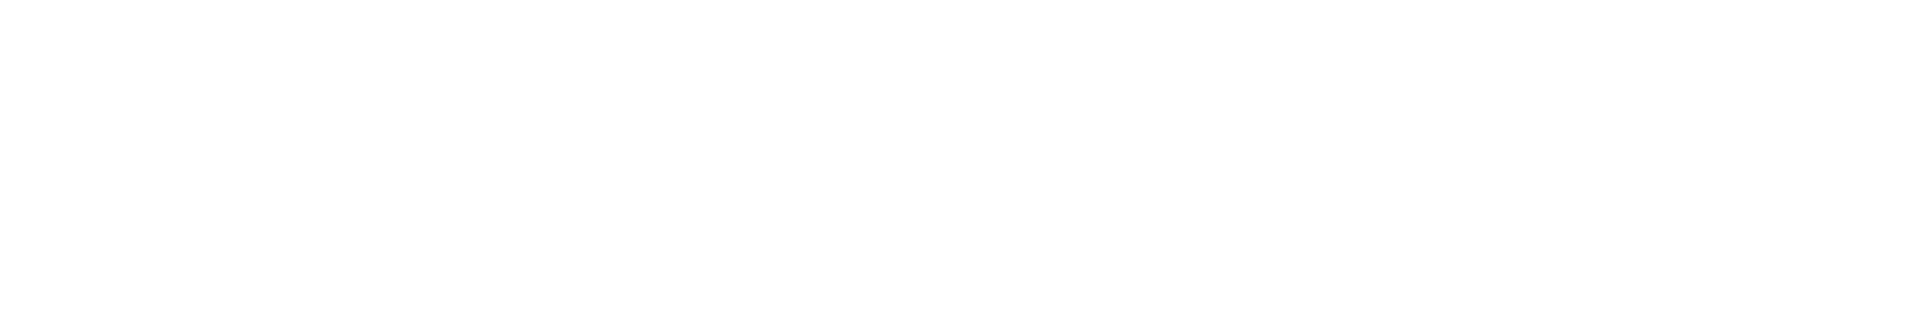
\includegraphics[scale=1.005]{mqtt4}\\\\